\documentclass{report}
\usepackage{pdfpages}
\usepackage[a4paper, top=2cm, bottom=2cm, left=2cm, right=2cm]{geometry}
\usepackage{fancyhdr}
\usepackage{amsmath} % Für mathematische Symbole
\usepackage{amssymb} % Für \mathbb
\usepackage[linesnumbered,ruled]{algorithm2e} % Für Algorithmus-Umgebung
\usepackage{ulem}
\usepackage{xcolor}
\usepackage{array}
\usepackage{graphicx}
\usepackage{listings}
\usepackage{xcolor}
\usepackage{naive-ebnf}
\usepackage[utf8]{inputenc}
\usepackage[absolute,overlay]{textpos}
\usepackage{tcolorbox}

\lstdefinestyle{cppstyle}{
    language=C++,             % Specify the language
    basicstyle=\ttfamily,     % Set the font to typewriter
    basicstyle=\ttfamily\footnotesize,
    keywordstyle=\color{blue}\bfseries, % Keywords in bold blue
    commentstyle=\color{green},         % Comments in green
    stringstyle=\color{red},            % Strings in red
    numbers=left,            % Line numbers on the left
    numberstyle=\tiny\color{gray}, % Line numbers in tiny gray font
    stepnumber=1,             % Line number step
    breaklines=true,          % Automatic line breaking
    tabsize=4,                % Set tab size
    showstringspaces=false,   % Don't show spaces in strings
    frame=single,             % Add a frame around the code
}

\newcommand{\name}{Marco Söllinger}
\newcommand{\fach}{SEN2}
\newcommand{\topic}{Übung 1}
\newcommand{\uebungangabe}{Uebung1.pdf}

\newcommand{\matnr}{s2410306011}
\newcommand{\uebungsgruppe}{Gruppe 1}
\newcommand{\aufwand}{2}


\pagestyle{fancy}
\normalem 
\fancyhead[R]{Marco Söllinger}  

\begin{document}
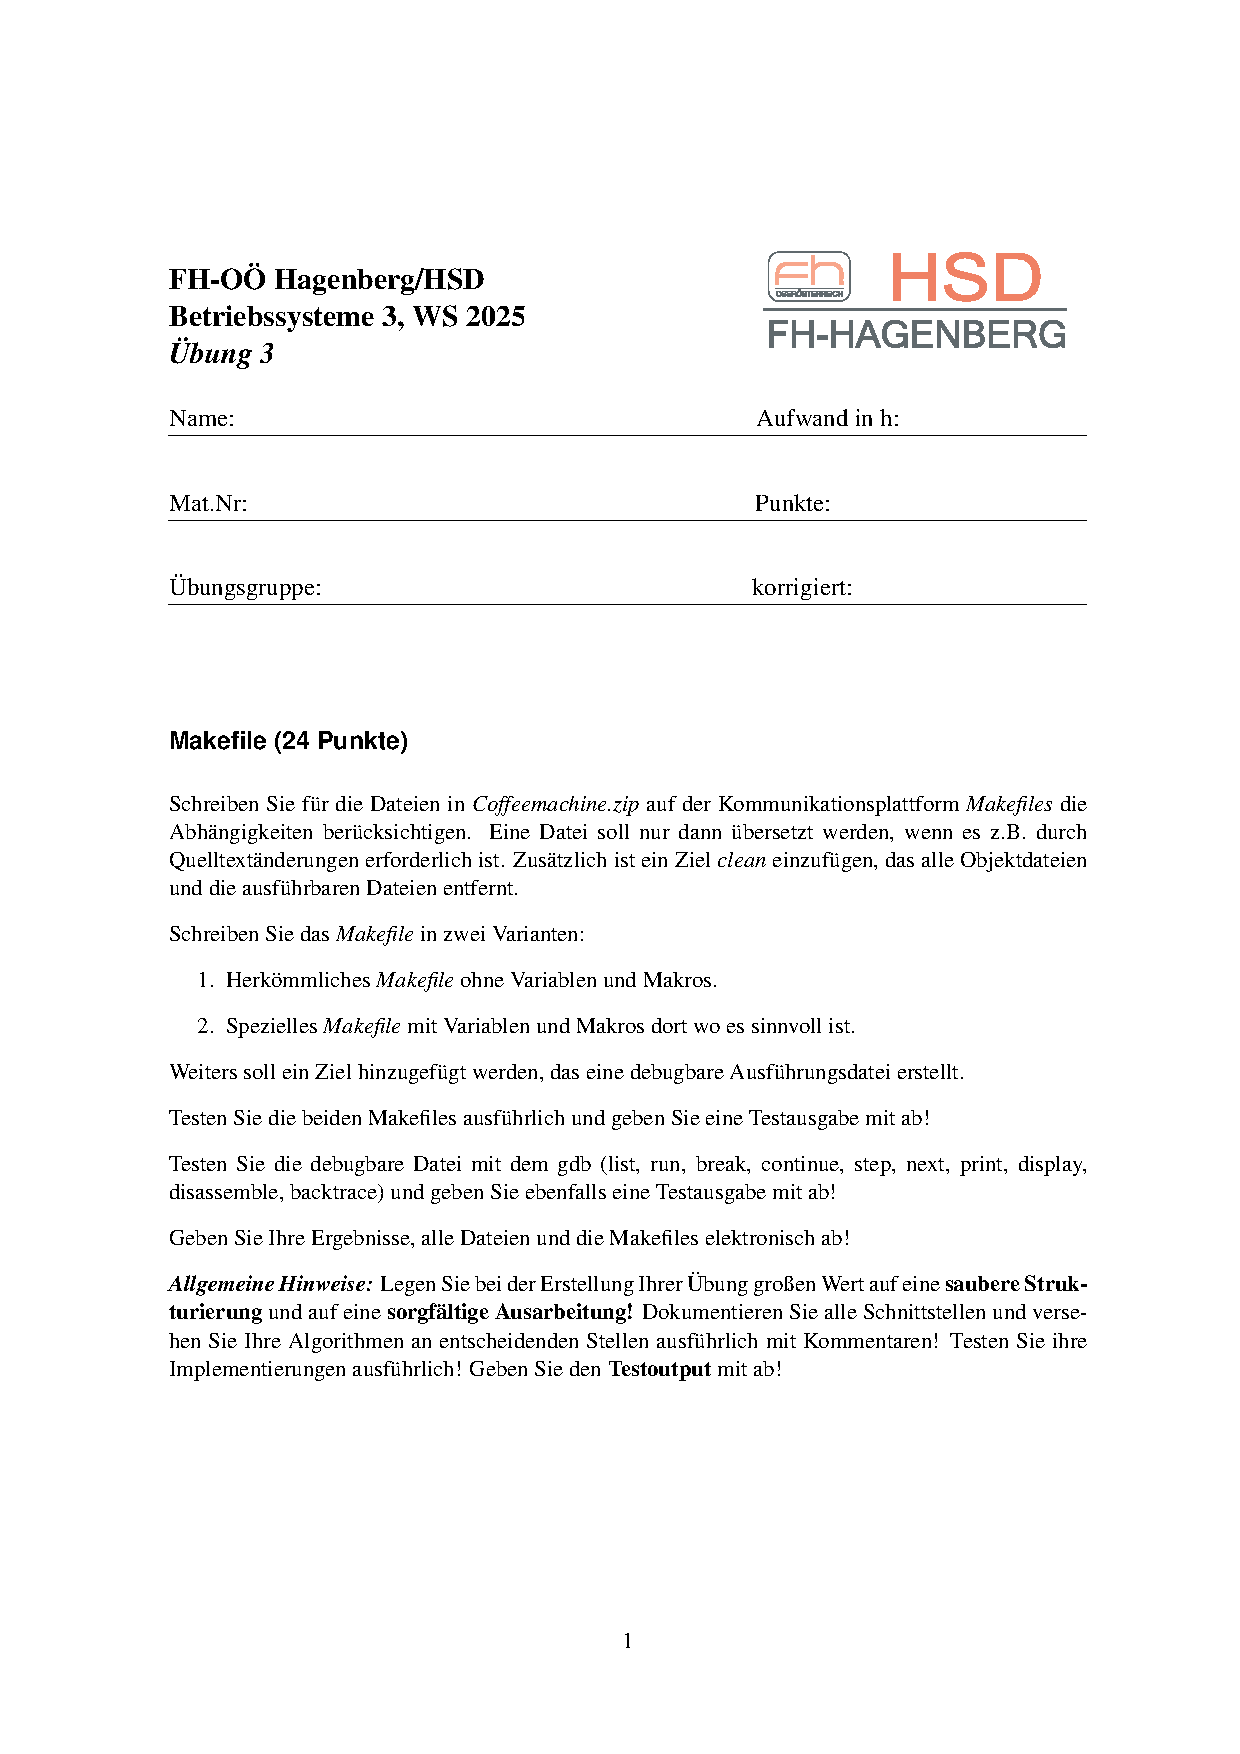
\includepdf[pages=1,pagecommand={
			\begin{textblock*}{5cm}(5.5cm, 6.9cm)
				\textbf{\name}
			\end{textblock*}
			\begin{textblock*}{5cm}(5.5cm, 8.4cm)
				\textbf{\matnr}
			\end{textblock*}
			\begin{textblock*}{5cm}(5.5cm, 9.8cm)
				\textbf{\uebungsgruppe}
			\end{textblock*}
			\begin{textblock*}{5cm}(15.3cm, 6.9cm)
				\textbf{\aufwand}
			\end{textblock*}
		}]{Uebung3.pdf}
%\includepdf[pages=2-]{Uebung2.pdf}

\section*{Beispiel 1}

\subsection*{1.1 Makefile simple}


\subsubsection*{1.1.1 Makefile\_1}

\lstinputlisting[style=cppstyle, title=\texttt{Makefile\_1} ]{../coffeemachine/Makefile_1}

\subsubsection*{1.1.2 Run build}

\begin{lstlisting}[style=cppstyle, title=\texttt{Terminal Output}]
flashfish@fedora ~/D/R/F/B/U/coffeemachine (main)> make -f Makefile_1
gcc -c coffeemachine_api.c -Wall -Wextra
coffeemachine_api.c: In function ‘grindCoffee’:
coffeemachine_api.c:38:16: warning: comparison of unsigned expression in ‘>= 0’ is always true [-Wtype-limits]
   38 |   if (_coffee_ >= 0) // see assumption in the SRD
      |                ^~
coffeemachine_api.c: In function ‘insertSugar’:
coffeemachine_api.c:52:15: warning: comparison of unsigned expression in ‘>= 0’ is always true [-Wtype-limits]
   52 |   if (_sugar_ >= 0) // see assumption in the SRD
      |               ^~
coffeemachine_api.c: In function ‘insertMilk’:
coffeemachine_api.c:66:14: warning: comparison of unsigned expression in ‘>= 0’ is always true [-Wtype-limits]
   66 |   if (_milk_ >= 0) // see assumption in the SRD
      |              ^~
coffeemachine_api.c: In function ‘brewCoffee’:
coffeemachine_api.c:80:15: warning: comparison of unsigned expression in ‘>= 0’ is always true [-Wtype-limits]
   80 |   if (_water_ >= 0) // see assumption in the SRD
      |               ^~
gcc -c coffeemachine_functionality.c -Wall -Wextra
coffeemachine_functionality.c: In function ‘changePrices’:
coffeemachine_functionality.c:155:28: warning: unused parameter ‘keymask’ [-Wunused-parameter]
  155 | void changePrices(unsigned keymask)
      |                   ~~~~~~~~~^~~~~~~
gcc -c coffeemachine_main.c -Wall -Wextra
gcc -o output *.o -Wall -Wextra
\end{lstlisting}

\subsubsection*{1.1.3 Run build again}

\begin{lstlisting}[style=cppstyle, title=\texttt{Terminal Output}]
flashfish@fedora ~/D/R/F/B/U/coffeemachine (main)> make -f Makefile_1
gcc -c coffeemachine_functionality.c -Wall -Wextra
coffeemachine_functionality.c: In function ‘changePrices’:
coffeemachine_functionality.c:155:28: warning: unused parameter ‘keymask’ [-Wunused-parameter]
  155 | void changePrices(unsigned keymask)
      |                   ~~~~~~~~~^~~~~~~
gcc -o output *.o -Wall -Wextra
\end{lstlisting}

\subsubsection*{1.1.4 Run clean}

\begin{lstlisting}[style=cppstyle, title=\texttt{Terminal Output}]
flashfish@fedora ~/D/R/F/B/U/coffeemachine (main)> make -f Makefile_1 clean
rm *.o output output_dbg
\end{lstlisting}


\subsubsection*{1.1.5 Run Run without build before}

\begin{lstlisting}[style=cppstyle, title=\texttt{Terminal Output}]
flashfish@fedora ~/D/R/F/B/U/coffeemachine (main)> make -f Makefile_1 run
gcc -c coffeemachine_api.c -Wall -Wextra
coffeemachine_api.c: In function ‘grindCoffee’:
coffeemachine_api.c:38:16: warning: comparison of unsigned expression in ‘>= 0’ is always true [-Wtype-limits]
   38 |   if (_coffee_ >= 0) // see assumption in the SRD
      |                ^~
coffeemachine_api.c: In function ‘insertSugar’:
coffeemachine_api.c:52:15: warning: comparison of unsigned expression in ‘>= 0’ is always true [-Wtype-limits]
   52 |   if (_sugar_ >= 0) // see assumption in the SRD
      |               ^~
coffeemachine_api.c: In function ‘insertMilk’:
coffeemachine_api.c:66:14: warning: comparison of unsigned expression in ‘>= 0’ is always true [-Wtype-limits]
   66 |   if (_milk_ >= 0) // see assumption in the SRD
      |              ^~
coffeemachine_api.c: In function ‘brewCoffee’:
coffeemachine_api.c:80:15: warning: comparison of unsigned expression in ‘>= 0’ is always true [-Wtype-limits]
   80 |   if (_water_ >= 0) // see assumption in the SRD
      |               ^~
gcc -c coffeemachine_functionality.c -Wall -Wextra
coffeemachine_functionality.c: In function ‘changePrices’:
coffeemachine_functionality.c:155:28: warning: unused parameter ‘keymask’ [-Wunused-parameter]
  155 | void changePrices(unsigned keymask)
      |                   ~~~~~~~~~^~~~~~~
gcc -c coffeemachine_main.c -Wall -Wextra
gcc -o output *.o -Wall -Wextra
./output
Coffee Machine> ^Cmake: *** [Makefile_1:32: run] Interrupt
\end{lstlisting}

\subsubsection*{1.1.6 Run debug build}

\begin{lstlisting}[style=cppstyle, title=\texttt{Terminal Output}]
flashfish@fedora ~/D/R/F/B/U/coffeemachine (main) [SIGINT]> make -f Makefile_1 output_dbg
gcc -c coffeemachine_api.c -g -O0 -Wall -Wextra -o coffeemachine_api.dbg.o
coffeemachine_api.c: In function ‘grindCoffee’:
coffeemachine_api.c:38:16: warning: comparison of unsigned expression in ‘>= 0’ is always true [-Wtype-limits]
   38 |   if (_coffee_ >= 0) // see assumption in the SRD
      |                ^~
coffeemachine_api.c: In function ‘insertSugar’:
coffeemachine_api.c:52:15: warning: comparison of unsigned expression in ‘>= 0’ is always true [-Wtype-limits]
   52 |   if (_sugar_ >= 0) // see assumption in the SRD
      |               ^~
coffeemachine_api.c: In function ‘insertMilk’:
coffeemachine_api.c:66:14: warning: comparison of unsigned expression in ‘>= 0’ is always true [-Wtype-limits]
   66 |   if (_milk_ >= 0) // see assumption in the SRD
      |              ^~
coffeemachine_api.c: In function ‘brewCoffee’:
coffeemachine_api.c:80:15: warning: comparison of unsigned expression in ‘>= 0’ is always true [-Wtype-limits]
   80 |   if (_water_ >= 0) // see assumption in the SRD
      |               ^~
gcc -c coffeemachine_functionality.c -g -O0 -Wall -Wextra -o coffeemachine_functionality.dbg.o
coffeemachine_functionality.c: In function ‘changePrices’:
coffeemachine_functionality.c:155:28: warning: unused parameter ‘keymask’ [-Wunused-parameter]
  155 | void changePrices(unsigned keymask)
      |                   ~~~~~~~~~^~~~~~~
gcc -c coffeemachine_main.c -g -O0 -Wall -Wextra -o coffeemachine_main.dbg.o
gcc -o output_dbg coffeemachine_api.dbg.o coffeemachine_functionality.dbg.o coffeemachine_main.dbg.o -Wall -Wextra
flashfish@fedora ~/D/R/F/B/U/coffeemachine (main)> gdb ./output_dbg
GNU gdb (Fedora Linux) 16.3-1.fc42
Copyright (C) 2024 Free Software Foundation, Inc.
License GPLv3+: GNU GPL version 3 or later <http://gnu.org/licenses/gpl.html>
This is free software: you are free to change and redistribute it.
There is NO WARRANTY, to the extent permitted by law.
Type "show copying" and "show warranty" for details.
This GDB was configured as "x86_64-redhat-linux-gnu".
Type "show configuration" for configuration details.
For bug reporting instructions, please see:
<https://www.gnu.org/software/gdb/bugs/>.
Find the GDB manual and other documentation resources online at:
    <http://www.gnu.org/software/gdb/documentation/>.

For help, type "help".
Type "apropos word" to search for commands related to "word"...
Reading symbols from ./output_dbg...
(gdb) exit
\end{lstlisting}


\subsubsection*{1.1.7 Run debug-run}

\begin{lstlisting}[style=cppstyle, title=\texttt{Terminal Output}]
flashfish@fedora ~/D/R/F/B/U/coffeemachine (main)> make -f Makefile_1 run-debug
gdb ./output_dbg
GNU gdb (Fedora Linux) 16.3-1.fc42
Copyright (C) 2024 Free Software Foundation, Inc.
License GPLv3+: GNU GPL version 3 or later <http://gnu.org/licenses/gpl.html>
This is free software: you are free to change and redistribute it.
There is NO WARRANTY, to the extent permitted by law.
Type "show copying" and "show warranty" for details.
This GDB was configured as "x86_64-redhat-linux-gnu".
Type "show configuration" for configuration details.
For bug reporting instructions, please see:
<https://www.gnu.org/software/gdb/bugs/>.
Find the GDB manual and other documentation resources online at:
    <http://www.gnu.org/software/gdb/documentation/>.

For help, type "help".
Type "apropos word" to search for commands related to "word"...
Reading symbols from ./output_dbg...
(gdb) exit
\end{lstlisting}

\subsubsection*{1.1.8 Test with gdb}

\begin{lstlisting}[style=cppstyle, title=\texttt{Terminal Output}]
flashfish@fedora ~/D/R/F/B/U/coffeemachine (main)> make -f Makefile_1 run-debug
gcc -c coffeemachine_api.c -g -O0 -Wall -Wextra -o coffeemachine_api.dbg.o
coffeemachine_api.c: In function ‘grindCoffee’:
coffeemachine_api.c:33:16: warning: comparison of unsigned expression in ‘>= 0’ is always true [-Wtype-limits]
   33 |   if (_coffee_ >= 0) // see assumption in the SRD
      |                ^~
coffeemachine_api.c: In function ‘insertSugar’:
coffeemachine_api.c:46:15: warning: comparison of unsigned expression in ‘>= 0’ is always true [-Wtype-limits]
   46 |   if (_sugar_ >= 0) // see assumption in the SRD
      |               ^~
coffeemachine_api.c: In function ‘insertMilk’:
coffeemachine_api.c:60:14: warning: comparison of unsigned expression in ‘>= 0’ is always true [-Wtype-limits]
   60 |   if (_milk_ >= 0) // see assumption in the SRD
      |              ^~
coffeemachine_api.c: In function ‘brewCoffee’:
coffeemachine_api.c:74:15: warning: comparison of unsigned expression in ‘>= 0’ is always true [-Wtype-limits]
   74 |   if (_water_ >= 0) // see assumption in the SRD
      |               ^~
gcc -c coffeemachine_functionality.c -g -O0 -Wall -Wextra -o coffeemachine_functionality.dbg.o
coffeemachine_functionality.c: In function ‘changePrices’:
coffeemachine_functionality.c:155:28: warning: unused parameter ‘keymask’ [-Wunused-parameter]
  155 | void changePrices(unsigned keymask)
      |                   ~~~~~~~~~^~~~~~~
gcc -c coffeemachine_main.c -g -O0 -Wall -Wextra -o coffeemachine_main.dbg.o
gcc -o output_dbg coffeemachine_api.dbg.o coffeemachine_functionality.dbg.o coffeemachine_main.dbg.o -Wall -Wextra
gdb ./output_dbg
GNU gdb (Fedora Linux) 16.3-1.fc42
Copyright (C) 2024 Free Software Foundation, Inc.
License GPLv3+: GNU GPL version 3 or later <http://gnu.org/licenses/gpl.html>
This is free software: you are free to change and redistribute it.
There is NO WARRANTY, to the extent permitted by law.
Type "show copying" and "show warranty" for details.
This GDB was configured as "x86_64-redhat-linux-gnu".
Type "show configuration" for configuration details.
For bug reporting instructions, please see:
<https://www.gnu.org/software/gdb/bugs/>.
Find the GDB manual and other documentation resources online at:
    <http://www.gnu.org/software/gdb/documentation/>.

For help, type "help".
Type "apropos word" to search for commands related to "word"...
Reading symbols from ./output_dbg...
(gdb) list activateCoffeeMachine
15
16      //----------------------------------------------------------------------
17      // The main function that activates the machine. Here the endless loop
18      // for the keyboard input dispatcher of the simulator is located.
19
20      void activateCoffeeMachine() {
21        unsigned char kbd_input = '\0';
22
23        for (;;) {
24          printf("Coffee Machine> ");
(gdb) b 24
Breakpoint 1 at 0x4004b2: file coffeemachine_api.c, line 24.
(gdb) run
Starting program: /home/flashfish/Documents/Repo/FH/BSY3/Uebung03/coffeemachine/output_dbg

This GDB supports auto-downloading debuginfo from the following URLs:
  <https://debuginfod.fedoraproject.org/>
Enable debuginfod for this session? (y or [n]) y
Debuginfod has been enabled.
To make this setting permanent, add 'set debuginfod enabled on' to .gdbinit.
[Thread debugging using libthread_db enabled]
Using host libthread_db library "/lib64/libthread_db.so.1".

Breakpoint 1, activateCoffeeMachine () at coffeemachine_api.c:24
24          printf("Coffee Machine> ");
(gdb) next
25          kbd_input = getchar();
(gdb) next
Coffee Machine> h
26          getchar(); // eat the newline character and ignore it
(gdb) next
27          dispatch(kbd_input);
(gdb) print kbd_input
$1 = 104 'h'
(gdb)
\end{lstlisting}




\subsection*{1.2 Makefile advanced}

\subsubsection*{1.2.1 Makefile\_2}

\lstinputlisting[style=cppstyle, title=\texttt{Makefile\_2} ]{../coffeemachine/Makefile_2}

\subsubsection*{1.2.2 Run build}

\begin{lstlisting}[style=cppstyle, title=\texttt{Terminal Output}]
flashfish@fedora ~/D/R/F/B/U/coffeemachine (main)> make -f Makefile_2
clang  -Wall -Wextra  -c coffeemachine_api.c -o coffeemachine_api.o
clang  -Wall -Wextra  -c coffeemachine_functionality.c -o coffeemachine_functionality.o
coffeemachine_functionality.c:155:28: warning: unused parameter 'keymask' [-Wunused-parameter]
  155 | void changePrices(unsigned keymask)
      |                            ^
1 warning generated.
clang  -Wall -Wextra  -c coffeemachine_main.c -o coffeemachine_main.o
clang -o output coffeemachine_api.o coffeemachine_functionality.o coffeemachine_main.o -Wall -Wextra
flashfish@fedora ~/D/R/F/B/U/coffeemachine (main)> ./output
Coffee Machine> ^C⏎
\end{lstlisting}

\subsubsection*{1.2.3 Run build again}

\begin{lstlisting}[style=cppstyle, title=\texttt{Terminal Output}]
flashfish@fedora ~/D/R/F/B/U/coffeemachine (main) [SIGINT]> make -f Makefile_2
make: 'output' is up to date.
\end{lstlisting}

\subsubsection*{1.2.4 Run clean}

\begin{lstlisting}[style=cppstyle, title=\texttt{Terminal Output}]
flashfish@fedora ~/D/R/F/B/U/coffeemachine (main) [2]> make -f Makefile_2 clean
rm -f *.o *.dbg.o output output_dbg
\end{lstlisting}


\subsubsection*{1.2.5 Run Run without build before}

\begin{lstlisting}[style=cppstyle, title=\texttt{Terminal Output}]
flashfish@fedora ~/D/R/F/B/U/coffeemachine (main)> make -f Makefile_2 run
clang  -Wall -Wextra  -c coffeemachine_api.c -o coffeemachine_api.o
clang  -Wall -Wextra  -c coffeemachine_functionality.c -o coffeemachine_functionality.o
coffeemachine_functionality.c:155:28: warning: unused parameter 'keymask' [-Wunused-parameter]
  155 | void changePrices(unsigned keymask)
      |                            ^
1 warning generated.
clang  -Wall -Wextra  -c coffeemachine_main.c -o coffeemachine_main.o
clang -o output coffeemachine_api.o coffeemachine_functionality.o coffeemachine_main.o -Wall -Wextra
./output
Coffee Machine> ^Cmake: *** [Makefile_2:28: run] Interrupt
\end{lstlisting}

\subsubsection*{1.2.6 Run debug build}

\begin{lstlisting}[style=cppstyle, title=\texttt{Terminal Output}]
flashfish@fedora ~/D/R/F/B/U/coffeemachine (main)> make -f Makefile_2 output_dbg
clang  -Wall -Wextra  -g -O0 -c coffeemachine_api.c -o coffeemachine_api.dbg.o
clang  -Wall -Wextra  -g -O0 -c coffeemachine_functionality.c -o coffeemachine_functionality.dbg.o
coffeemachine_functionality.c:155:28: warning: unused parameter 'keymask' [-Wunused-parameter]
  155 | void changePrices(unsigned keymask)
      |                            ^
1 warning generated.
clang  -Wall -Wextra  -g -O0 -c coffeemachine_main.c -o coffeemachine_main.dbg.o
clang -o output_dbg coffeemachine_api.dbg.o coffeemachine_functionality.dbg.o coffeemachine_main.dbg.o -Wall -Wextra
flashfish@fedora ~/D/R/F/B/U/coffeemachine (main)> gdb ./output_dbg
GNU gdb (Fedora Linux) 16.3-1.fc42
Copyright (C) 2024 Free Software Foundation, Inc.
License GPLv3+: GNU GPL version 3 or later <http://gnu.org/licenses/gpl.html>
This is free software: you are free to change and redistribute it.
There is NO WARRANTY, to the extent permitted by law.
Type "show copying" and "show warranty" for details.
This GDB was configured as "x86_64-redhat-linux-gnu".
Type "show configuration" for configuration details.
For bug reporting instructions, please see:
<https://www.gnu.org/software/gdb/bugs/>.
Find the GDB manual and other documentation resources online at:
    <http://www.gnu.org/software/gdb/documentation/>.

For help, type "help".
Type "apropos word" to search for commands related to "word"...
Reading symbols from ./output_dbg...
(gdb) exit
\end{lstlisting}


\subsubsection*{1.2.7 Run debug-run}

\begin{lstlisting}[style=cppstyle, title=\texttt{Terminal Output}]
flashfish@fedora ~/D/R/F/B/U/coffeemachine (main)> make -f Makefile_2 run-debug
clang  -Wall -Wextra  -g -O0 -c coffeemachine_api.c -o coffeemachine_api.dbg.o
clang  -Wall -Wextra  -g -O0 -c coffeemachine_functionality.c -o coffeemachine_functionality.dbg.o
coffeemachine_functionality.c:155:28: warning: unused parameter 'keymask' [-Wunused-parameter]
  155 | void changePrices(unsigned keymask)
      |                            ^
1 warning generated.
clang  -Wall -Wextra  -g -O0 -c coffeemachine_main.c -o coffeemachine_main.dbg.o
clang -o output_dbg coffeemachine_api.dbg.o coffeemachine_functionality.dbg.o coffeemachine_main.dbg.o -Wall -Wextra
gdb ./output_dbg
GNU gdb (Fedora Linux) 16.3-1.fc42
Copyright (C) 2024 Free Software Foundation, Inc.
License GPLv3+: GNU GPL version 3 or later <http://gnu.org/licenses/gpl.html>
This is free software: you are free to change and redistribute it.
There is NO WARRANTY, to the extent permitted by law.
Type "show copying" and "show warranty" for details.
This GDB was configured as "x86_64-redhat-linux-gnu".
Type "show configuration" for configuration details.
For bug reporting instructions, please see:
<https://www.gnu.org/software/gdb/bugs/>.
Find the GDB manual and other documentation resources online at:
    <http://www.gnu.org/software/gdb/documentation/>.

For help, type "help".
Type "apropos word" to search for commands related to "word"...
Reading symbols from ./output_dbg...
(gdb) exit
\end{lstlisting}

\subsubsection*{1.2.8 Test with gdb}

\begin{lstlisting}[style=cppstyle, title=\texttt{Terminal Output}]
flashfish@fedora ~/D/R/F/B/U/coffeemachine (main)> gdb ./output_dbg
GNU gdb (Fedora Linux) 16.3-1.fc42
Copyright (C) 2024 Free Software Foundation, Inc.
License GPLv3+: GNU GPL version 3 or later <http://gnu.org/licenses/gpl.html>
This is free software: you are free to change and redistribute it.
There is NO WARRANTY, to the extent permitted by law.
Type "show copying" and "show warranty" for details.
This GDB was configured as "x86_64-redhat-linux-gnu".
Type "show configuration" for configuration details.
For bug reporting instructions, please see:
<https://www.gnu.org/software/gdb/bugs/>.
Find the GDB manual and other documentation resources online at:
    <http://www.gnu.org/software/gdb/documentation/>.

For help, type "help".
Type "apropos word" to search for commands related to "word"...
Reading symbols from ./output_dbg...
(gdb) list
2
3       #include "coffeemachine_api.h"
4
5       //----------------------------------------------------------------------
6       int main()
7       {
8         activateCoffeeMachine();
9         return 0;
10      }
11
(gdb) b 8
Breakpoint 1 at 0x400f0f: file coffeemachine_main.c, line 8.
(gdb) run
Starting program: /home/flashfish/Documents/Repo/FH/BSY3/Uebung03/coffeemachine/output_dbg

This GDB supports auto-downloading debuginfo from the following URLs:
  <https://debuginfod.fedoraproject.org/>
Enable debuginfod for this session? (y or [n]) y
Debuginfod has been enabled.
To make this setting permanent, add 'set debuginfod enabled on' to .gdbinit.
[Thread debugging using libthread_db enabled]
Using host libthread_db library "/lib64/libthread_db.so.1".

Breakpoint 1, main () at coffeemachine_main.c:8
8         activateCoffeeMachine();
(gdb) step
activateCoffeeMachine () at coffeemachine_api.c:21
21        unsigned char kbd_input = '\0';
(gdb) list
16      //----------------------------------------------------------------------
17      // The main function that activates the machine. Here the endless loop
18      // for the keyboard input dispatcher of the simulator is located.
19
20      void activateCoffeeMachine() {
21        unsigned char kbd_input = '\0';
22
23        for (;;) {
24          printf("Coffee Machine> ");
25          kbd_input = getchar();
(gdb) step
24          printf("Coffee Machine> ");
(gdb) print kbd_input
$1 = 0 '\000'
\end{lstlisting}




\end{document}
